\subsection{Opgave 56}

Grafen for en funktion 

\begin{align*}
    f(x) = \frac{1}{4}x^2 + x + 2
\end{align*}

afgrænser sammed med x-aksen et område i intervallet [-4;2].

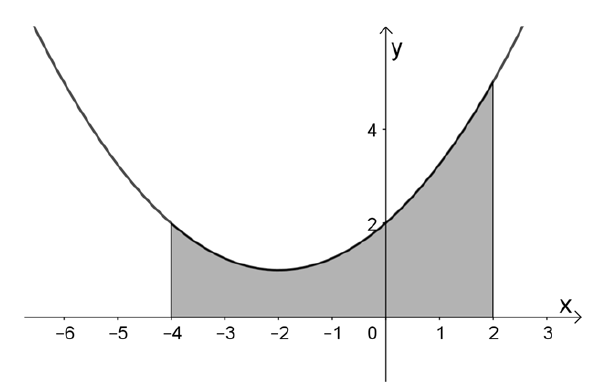
\includegraphics[width=8cm]{Opgave_51-56/Opgave_56/56.png}

Opstil et integral til bestemmelse af områdets areal.

\ans

For at opstille et integral på formen 

\begin{align*}
    \int_a^b f(x) dx
\end{align*}

skal vi bruge a og b værdierne og $f(x)$. Da området er i intervallet [-4;2] har vi $a = -4$ og $b = 2$.
Integralet bliver derfor

\begin{align*}
    \int_{-4}^{2} \frac{1}{4}x^2 + x + 2 dx
\end{align*}



